\documentclass[12pt,a4paper]{article}

\usepackage[utf8]{inputenc}
\usepackage[T1]{fontenc}
\usepackage{lmodern}
\usepackage{amsmath,amssymb,amsfonts}
\usepackage{amsthm}
\usepackage{graphicx}
\usepackage{booktabs}
\usepackage{array}
\usepackage{tabularx}
\usepackage{ragged2e}
\usepackage{hyperref}
\usepackage{geometry}
\usepackage{xcolor}
\usepackage{enumitem}
\usepackage{caption}
\usepackage{float}
\usepackage{url}
\usepackage{microtype}
\usepackage{setspace}
\usepackage{fancyhdr}
\usepackage{algorithm}
\usepackage{algpseudocode}
\usepackage{appendix}
\usepackage{tocloft}
\usepackage{tikz}
\usetikzlibrary{arrows.meta,positioning,calc,fit}
\usepackage{pgfplots}
\pgfplotsset{compat=1.17}
\pgfplotsset{every axis/.append style={font=\footnotesize}}

\setcounter{tocdepth}{2}
\renewcommand{\cftbeforesecskip}{3pt}
\setlength{\cftparskip}{0pt}
\setlength{\cftsubsecindent}{1.5em}
\setlength{\cftsecindent}{0em}

\geometry{a4paper, margin=2.5cm}

\linespread{1.08}
\setlength{\headheight}{14pt}
\emergencystretch=2em
\setlength{\parskip}{3pt}

\setlength{\aboverulesep}{2.5pt}
\setlength{\belowrulesep}{2.5pt}
\setlength{\extrarowheight}{2pt}

\captionsetup{font=small, labelfont=bf, textfont=it, skip=6pt}

\hypersetup{
    colorlinks=true,
    linkcolor=blue!70!black,
    citecolor=blue!70!black,
    urlcolor=blue!70!black,
    pdftitle={UniMind: A Middleware Framework for Bridging Classical AI Workloads and Quantum Computing Backends},
    pdfauthor={Y. X. Tan}
}

\newtheorem{definition}{Definition}[section]

\pagestyle{fancy}
\fancyhf{}
\fancyhead[L]{\small\itshape UniMind: A Middleware Framework}
\fancyhead[R]{\small\thepage}
\renewcommand{\headrulewidth}{0.4pt}

\floatname{algorithm}{Algorithm}

\newcommand{\umcheck}{\checkmark}
\newcommand{\umcross}{$\times$}

\begin{document}

\begin{titlepage}
\centering
\vspace*{2cm}

{\LARGE\bfseries UniMind: A Middleware Framework for\\[6pt]
Bridging Classical AI Workloads and\\[6pt]
Quantum Computing Backends\par}

\vspace{0.8cm}

{\normalsize\rmfamily Version 2.0 (August 23, 2026)\par}

\vspace{1.2cm}

{\Large Y. X. Tan\par}
\vspace{0.3cm}
{\normalsize\itshape Independent Researcher\par}
{\normalsize\itshape Email: yxtan5022@gmail.com\par}

\vspace{1.8cm}

{\large\bfseries Abstract\par}
\vspace{0.5cm}

\begin{minipage}{0.92\textwidth}
\small
As quantum computing transitions from theoretical research to practical deployment, a compatibility gap emerges between classical AI software stacks and probabilistic quantum hardware. Existing quantum machine learning frameworks operate at the application level and lack system-level abstractions for hardware adaptation, workload routing, and dynamic code generation. This paper presents \textbf{UniMind}, a middleware framework designed to reduce the abstraction gap between classical AI workloads and heterogeneous quantum-classical computing backends. UniMind introduces two components: (1)~an \textbf{LLM-driven orchestration layer} that interprets high-level task specifications and generates topology-aware execution plans through constrained sampling, operating exclusively in user space with sandboxed validation and rule-based fallback; and (2)~\textbf{Unibit}, a classical preprocessing representation based on sliding-window frequency estimation and sinc-based smoothing that produces parameters for standard quantum angle encoding. We implement a multi-backend mapping engine and validate the framework with reproducible experiments: mathematical correctness (empirical measurement probabilities converge to theoretical weights across 8192 shots, maximum $\langle Z \rangle$ deviation of $0.0110$), system performance (up to $10.9\times$ speedup via vectorized C-backend execution and $4.5\times$ end-to-end speedup via the Rust FFI engine, with a component-level breakdown attributing the residual overhead to Python-side normalization and marshaling), a three-arm baseline comparison against bare Qiskit and a rule-based dispatcher (only the UniMind pipeline covers all five benchmark task classes), an LLM-reliability benchmark (success rate 91.7--100\% across injected LLM quality levels, measured at $n{=}200$ per level with Wilson confidence intervals, with $100\%$ rejection of all adversarial intents), fault-injection analysis (four of five fault classes recovered in sub-millisecond detection time; one exposes a real robustness gap), a noise-sensitivity analysis quantifying the encoding's degradation under depolarizing and $T_1$ channels, a sandbox security evaluation (20 of 21 escape attempts blocked), and physical QPU validation on IBM hardware (\texttt{ibm\_marrakesh}): a placement-controlled QPU sweep on \texttt{ibm\_marrakesh} in which the bare encoding meets the $0.05$ tolerance across weights $w \in [0.05, 0.95]$ when the layout is pinned to a well-calibrated qubit (maximum $\langle Z \rangle$ deviation $0.028$), while an adversarially chosen qubit with $82\%$ readout error inflates distortion to $0.213$ --- establishing that single-qubit encoding fidelity on real hardware is dominated by placement and calibration state rather than by the encoding itself, with a two-parameter affine channel model $P_{\mathrm{obs}} = b + a\,w$ fitting every condition at shot-noise level; a component ablation attributing up to $+34$ points of success rate to the self-healing layer and showing that rule-based fallback reaches $100\%$ recovery under availability stress once template coverage is complete; and a path-decomposition calculus demonstrating that end-to-end reliability does not compose multiplicatively across stages that share the LLM (an empirically measured correlation penalty). We discuss the remaining limitations---notably deeper hardware error mitigation and cross-framework comparison---and propose a phased roadmap for quantum-ready AI middleware.
\end{minipage}

\vspace{0.8cm}

\noindent\textbf{Keywords:} Quantum Computing, AI Middleware, Angle Encoding, Hybrid Quantum-Classical Systems, LLM Orchestration, Unibit

\vfill

{\small\copyright\ 2026 Y. X. Tan. This work is licensed under CC BY 4.0; the accompanying software (\texttt{unimind-os}) is MIT-licensed.}

\vspace{0.4cm}

{\small\itshape Name-disambiguation note: the name ``UniMind'' is also used by an unrelated prior work on LLM-based multi-task brain decoding~\cite{lu2025unimind}; the present work is not affiliated with that work.\par}

\end{titlepage}

\tableofcontents
\newpage

\section{Introduction}

The rapid advancement of quantum computing hardware has introduced a growing mismatch between the capabilities of emerging quantum processors and the software infrastructure available to utilize them. Modern AI systems---deep learning models, reinforcement learning agents, and large language models---are built upon software stacks designed for deterministic, von Neumann architectures. Operating systems such as Linux, Windows, and macOS manage discrete binary states through priority-based schedulers, static device drivers, and predictable memory hierarchies~\cite{tanenbaum2023}. These assumptions are fundamentally incompatible with the probabilistic, measurement-driven execution model of quantum computers.

Current approaches to quantum machine learning (QML), including frameworks such as PennyLane~\cite{bergholm2018}, TensorFlow Quantum, and Qiskit Machine Learning, provide algorithm-level abstractions for constructing and training quantum circuits. However, these frameworks operate within existing classical operating systems and do not address system-level challenges such as dynamic hardware discovery, workload routing across heterogeneous backends, or intent-driven task orchestration. As quantum hardware diversifies---spanning superconducting qubits, trapped ions, photonic systems, and GPU-accelerated simulators~\cite{microsoft2024,aws2024}---the need for a unified middleware layer becomes increasingly apparent.

This paper presents \textbf{UniMind}, a middleware framework that addresses this gap. UniMind is not an operating system; it operates as a user-space orchestration layer atop existing classical operating systems. Its design is motivated by three observations:

\begin{enumerate}[leftmargin=2em]
    \item \textbf{Hardware heterogeneity is increasing.} AI workloads must increasingly target diverse backends (CPUs, GPUs, QPUs, simulators), each with distinct programming models and performance characteristics.
    \item \textbf{Intent-driven computing is emerging.} Large language models can translate natural language specifications into executable code, potentially reducing the barrier to programming heterogeneous systems~\cite{wang2024}.
    \item \textbf{Classical-to-quantum data encoding remains manual.} Translating classical data into quantum states typically requires hand-crafted encoding circuits, creating friction in hybrid workflows.
\end{enumerate}

UniMind addresses these observations through three components:

\begin{itemize}
    \item An \textbf{LLM-driven orchestration layer} (Section~\ref{sec:orchestrator}) that interprets task specifications and generates execution plans, subject to sandboxed validation and deterministic fallback mechanisms.
    \item \textbf{Unibit} (Section~\ref{sec:unibit}), a classical preprocessing representation that computes sliding-window frequency estimates over binary sequences, producing parameters suitable for standard quantum angle encoding.
    \item A \textbf{multi-backend quantum mapping engine} (Section~\ref{sec:bridge}) that translates Unibit parameters into parameterized quantum circuits and routes execution to available backends.
\end{itemize}

The main contributions of this paper are:

\begin{enumerate}[leftmargin=2em]
    \item We identify system-level gaps between classical AI software stacks and quantum computing hardware that are not addressed by existing QML frameworks.
    \item We propose UniMind, a middleware framework with an LLM-driven orchestration layer, a classical preprocessing representation (Unibit), and a multi-backend quantum mapping engine.
    \item We present a functional proof-of-concept implementation in C++, Rust, and Python, with \textbf{quantitative validation}: mathematical verification via 8192-shot measurement convergence ($\langle Z \rangle$ deviation $= 0.0110$), performance micro-benchmarks demonstrating up to $10.9\times$ speedup via vectorized C-backend execution and $4.5\times$ end-to-end speedup via Rust FFI (with a component-level latency breakdown), a three-arm baseline comparison, an LLM-reliability benchmark, fault-injection analysis, a noise-sensitivity study, a sandbox security evaluation, and placement-controlled physical QPU sweeps on \texttt{ibm\_marrakesh} (bare encoding within tolerance on calibrated layouts, max.\ deviation $0.028$; adversarial placement inflates distortion to $0.213$), an architectural ablation, an instrumented failure taxonomy, and a reliability-composition calculus.
    \item We provide an honest, experiment-backed assessment of limitations---including LLM reliability, quantum noise sensitivity, and the security of LLM-generated code---and outline the experiments still required for future validation.
    \item We propose a phased roadmap for the development of quantum-ready AI middleware.
\end{enumerate}

\paragraph{Scope and limitations.} This paper presents a system design and proof-of-concept implementation. We do not claim quantum advantage, novel quantum algorithms, or comprehensive end-to-end system evaluation. The Unibit-to-qubit mapping is an instance of standard angle encoding~\cite{schuld2021}; our contribution lies in the classical preprocessing pipeline and the multi-backend orchestration layer, not in the quantum circuit design itself.

The remainder of this paper is organized as follows. Section~\ref{sec:background} provides background. Section~\ref{sec:architecture} presents the UniMind architecture. Section~\ref{sec:implementation} describes the implementation. Section~\ref{sec:evaluation} presents quantitative evaluation with real experimental data. Section~\ref{sec:discussion} discusses limitations, threats to validity, and a roadmap. Section~\ref{sec:conclusion} concludes.


\section{Background}\label{sec:background}

\subsection{Classical Operating Systems and AI}

Modern operating systems are designed around the von Neumann architecture, where a central processing unit sequentially fetches, decodes, and executes instructions from memory~\cite{tanenbaum2023}. The OS kernel manages hardware resources through device drivers, process schedulers, and memory managers, providing a stable abstraction layer for user-space applications.

AI workloads, particularly deep learning, operate within this paradigm. Neural networks are represented as computational graphs of matrix multiplications and nonlinear activations, executed on CPUs, GPUs, or specialized accelerators. The software stack assumes deterministic, sequential execution with well-defined memory addresses.

This paradigm presents three limitations for quantum-era computing:

\begin{enumerate}[leftmargin=2em]
    \item \textbf{Binary rigidity.} Classical bits exist in exactly one of two states (0 or 1), whereas quantum computation manipulates continuous probability amplitudes.
    \item \textbf{Deterministic scheduling.} Classical OS schedulers assume predictable execution times, incompatible with probabilistic, shot-based quantum execution.
    \item \textbf{Static hardware abstraction.} Traditional device drivers cannot dynamically adapt to heterogeneous quantum-classical hybrid systems.
\end{enumerate}

\subsection{Quantum Computing Fundamentals}

Quantum computing leverages quantum mechanical principles to process information. The fundamental unit is the \textbf{qubit}:
\begin{equation}
    |\psi\rangle = \alpha|0\rangle + \beta|1\rangle
\end{equation}
where $\alpha, \beta \in \mathbb{C}$ satisfy $|\alpha|^2 + |\beta|^2 = 1$.

Quantum operations are performed through \textbf{quantum gates}. Key gates include:
\begin{itemize}
    \item \textbf{Pauli-X gate:} $X = \begin{pmatrix} 0 & 1 \\ 1 & 0 \end{pmatrix}$ (bit flip)
    \item \textbf{Y-rotation gate:} $R_y(\theta) = \begin{pmatrix} \cos(\theta/2) & -\sin(\theta/2) \\ \sin(\theta/2) & \cos(\theta/2) \end{pmatrix}$
    \item \textbf{Hadamard gate:} $H = \frac{1}{\sqrt{2}}\begin{pmatrix} 1 & 1 \\ 1 & -1 \end{pmatrix}$
\end{itemize}

A quantum circuit applies a sequence of gates to a qubit register, followed by measurement that collapses the state into classical bits according to the Born rule.

Current hardware operates in the \textbf{NISQ} era~\cite{preskill2018}, characterized by 50--1000 qubits, high gate error rates, and short coherence times. Prominent quantum algorithms include Shor's factoring algorithm~\cite{shor1994} and variational quantum eigensolvers~\cite{kandala2017}, and quantum machine learning has been surveyed extensively~\cite{biamonte2017,cerezo2021}.

\subsection{The Gap: Why Current Systems Are Not Quantum-Ready}

\begin{table}[H]
\centering
\caption{Classical vs. Quantum Computing Paradigms}
\label{tab:comparison}
\small
\begin{tabular}{@{}lll@{}}
\toprule
\textbf{Aspect} & \textbf{Classical} & \textbf{Quantum} \\
\midrule
Data unit & Bit (0 or 1) & Qubit ($\alpha|0\rangle + \beta|1\rangle$) \\
Operation & Deterministic logic gates & Unitary transformations \\
Scheduling & Priority-based, deterministic & Probabilistic, shot-based \\
Error model & Bit-flip detection & Decoherence, gate noise \\
Software role & Resource management & Circuit compilation + state mgmt. \\
\bottomrule
\end{tabular}
\end{table}

No existing operating system provides native support for quantum state management, probabilistic scheduling, or dynamic circuit compilation. This gap motivates the UniMind middleware framework.


\section{UniMind Framework Architecture}\label{sec:architecture}

Figure~\ref{fig:architecture} presents the system architecture. UniMind is organized as three cooperating layers, all operating in user space atop a classical host OS: (i)~the \textbf{AI-as-Orchestrator} planning layer (Section~\ref{sec:orchestrator}), which interprets natural-language intents, generates candidate code under a three-stage validation pipeline, and falls back to a rule-based dispatcher when LLM inference fails; (ii)~a pair of \textbf{middleware services}---topology-aware hardware detection and the accelerated Unibit engine (Section~\ref{sec:implementation})---that supply system context and fast classical preprocessing to both upper and lower layers; and (iii)~the \textbf{multi-backend quantum bridge} (Section~\ref{sec:bridge}), which exposes a unified API over classical simulation, Qiskit/AerSimulator, CUDA-Q, and IBM Quantum hardware. The subsections below describe each layer from design down to implementation.

\begin{figure}[t]
\centering
\resizebox{0.97\textwidth}{!}{%
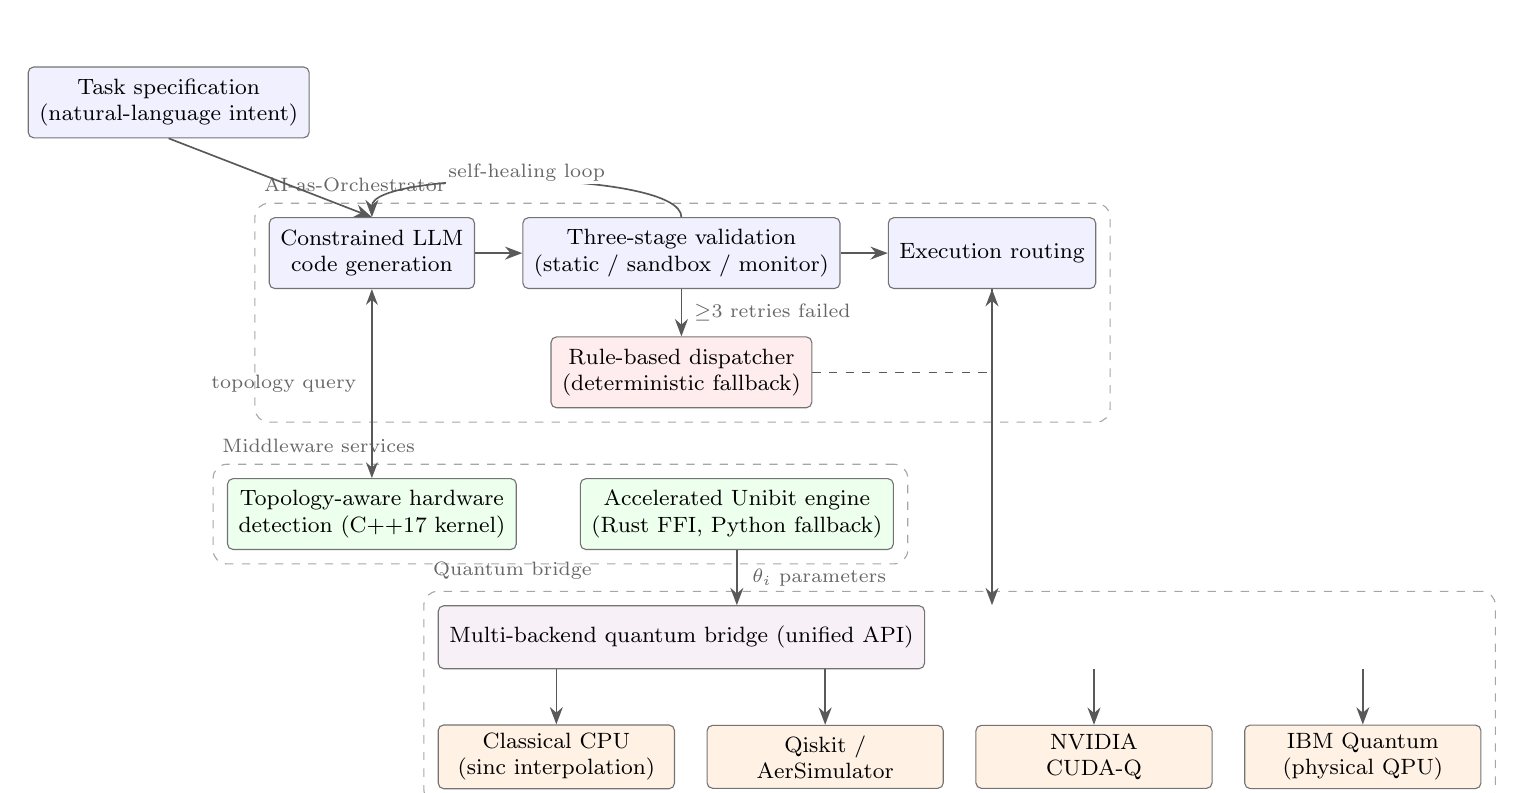
\begin{tikzpicture}[
  font=\footnotesize,
  comp/.style={draw=black!55, fill=blue!6, rounded corners=2pt, align=center, minimum height=9mm, inner sep=4pt},
  svc/.style={draw=black!55, fill=green!7, rounded corners=2pt, align=center, minimum height=9mm, inner sep=4pt},
  be/.style={draw=black!55, fill=orange!10, rounded corners=2pt, align=center, minimum height=8mm, inner sep=3pt},
  fb/.style={draw=black!55, fill=red!7, rounded corners=2pt, align=center, minimum height=9mm, inner sep=4pt},
  lay/.style={draw=black!35, dashed, rounded corners=5pt},
  arr/.style={-{Stealth[length=2.2mm]}, semithick, black!65},
  lab/.style={font=\scriptsize, text=black!60}]
\node[comp] (intent) {Task specification\\(natural-language intent)};
\node[comp, below left=10mm and -21mm of intent.south east] (gen) {Constrained LLM\\code generation};
\node[comp, right=6mm of gen] (valid) {Three-stage validation\\(static / sandbox / monitor)};
\node[comp, right=6mm of valid] (route) {Execution routing};
\node[fb, below=6mm of valid] (fallback) {Rule-based dispatcher\\(deterministic fallback)};
\node[svc, below=24mm of gen] (detect) {Topology-aware hardware\\detection (C++17 kernel)};
\node[svc, right=8mm of detect] (engine) {Accelerated Unibit engine\\(Rust FFI, Python fallback)};
\node[comp, fill=violet!6, minimum height=8mm, inner sep=4pt, below=25mm of fallback] (api) {Multi-backend quantum bridge (unified API)};
\node[be, below=7mm of api.south west, anchor=north west, minimum width=30mm] (cpu) {Classical CPU\\(sinc interpolation)};
\node[be, right=4mm of cpu, minimum width=30mm] (aer) {Qiskit /\\AerSimulator};
\node[be, right=4mm of aer, minimum width=30mm] (cudaq) {NVIDIA\\CUDA-Q};
\node[be, right=4mm of cudaq, minimum width=30mm] (ibm) {IBM Quantum\\(physical QPU)};
\node[lay, fit=(gen)(valid)(route)(fallback), inner sep=5pt] (layorc) {};
\node[lab, anchor=south west] at ([yshift=0.5pt]layorc.north west) {AI-as-Orchestrator};
\node[lay, fit=(detect)(engine), inner sep=5pt] (laysvc) {};
\node[lab, anchor=south west] at ([yshift=0.5pt]laysvc.north west) {Middleware services};
\node[lay, fit=(api)(cpu)(ibm), inner sep=5pt] (laybrd) {};
\node[lab, anchor=south west] at ([yshift=0.5pt]laybrd.north west) {Quantum bridge};
\draw[arr] (intent.south) -- (gen.north);
\draw[arr] (gen) -- (valid);
\draw[arr] (valid) -- (route);
\draw[arr] (valid.south) -- node[lab, right=1pt] {$\ge$3 retries failed} (fallback.north);
\draw[arr, dashed] (fallback.east) -| (route.south);
\draw[arr] (valid.north) .. controls +(0,0.6cm) and +(0,0.6cm) .. node[lab, above=-1pt, fill=white, inner sep=1pt] {self-healing loop} (gen.north);
\draw[{Stealth[length=2mm]}-{Stealth[length=2mm]}, semithick, black!65] (gen.south) -- node[lab, left=2pt] {topology query} (detect.north);
\draw[arr] (route.south) -- (route.south|-api.north);
\draw[arr] (engine.south) -- node[lab, right=2pt] {$\theta_i$ parameters} (engine.south|-api.north);
\foreach \b in {cpu,aer,cudaq,ibm}
  \draw[arr] (api.south-|\b.north) -- (\b.north);
\end{tikzpicture}}
\caption{UniMind system architecture. The orchestrator plans tasks entirely in user space with sandboxed validation and a deterministic rule-based fallback; middleware services provide topology context and accelerated Unibit preprocessing; the quantum bridge routes validated workloads across heterogeneous backends through a unified API.}
\label{fig:architecture}
\end{figure}

\subsection{AI-as-Orchestrator: LLM-Driven Intent Interpretation Layer}\label{sec:orchestrator}

We explicitly reject the notion of placing an LLM within the OS kernel. Traditional kernels require microsecond-level deterministic response times; LLM inference requires hundreds of milliseconds and is inherently non-deterministic.

Instead, UniMind introduces an \textbf{AI-as-Orchestrator} layer that resides entirely in user space, functioning as an asynchronous planning agent for coarse-grained task planning.

The orchestration pipeline operates as follows:

\begin{enumerate}[leftmargin=2em]
    \item \textbf{Intent reception.} A user or agent provides a natural language task specification.
    \item \textbf{Topology query.} The orchestrator queries the hardware detection module for current system information.
    \item \textbf{Constrained code generation.} The LLM generates candidate code, constrained by a system prompt specifying permitted APIs and output format.
    \item \textbf{Three-stage validation.} Generated code must pass: (a)~static analysis against a whitelist; (b)~sandboxed compilation; (c)~runtime monitoring with watchdog termination.
    \item \textbf{Execution routing.} Validated code is dispatched to the appropriate backend.
    \item \textbf{Deterministic fallback.} If LLM inference fails after three retry attempts, the system falls back to a \textbf{rule-based dispatcher} that maps intents to predefined circuit templates (e.g., Bell state preparation for entanglement tasks, variational ansatz templates for classification tasks).
\end{enumerate}

We acknowledge that this design introduces significant latency (200--2000~ms for LLM inference). The orchestrator is therefore positioned as a \textbf{task planner}, not a \textbf{task executor}.

\subsection{Unibit: A Sliding-Window Amplitude Proxy}\label{sec:unibit}

The Unibit is a \textbf{classical} preprocessing representation that produces parameters suitable for quantum angle encoding.

\begin{definition}[Unibit Weight]
Given a binary sequence $B = \{b_1, b_2, \dots, b_n\}$ where $b_i \in \{0, 1\}$, the Unibit weight at position $i$ is the local frequency of ones within a sliding window:
\begin{equation}
    w_i = \frac{1}{|W_i|} \sum_{j \in W_i} b_j, \quad W_i = [\max(1, i - \Delta),\; \min(n, i + \Delta)]
\end{equation}
where $\Delta$ is the half-window size (default: $\Delta = 2$, yielding a 5-bit window). This yields $w_i \in [0, 1]$.
\end{definition}

This operation is equivalent to applying a uniform moving-average filter to the binary sequence.

\begin{definition}[Folding]
The folding operation maps each weight to a continuous signal value via sinc interpolation:
\begin{equation}
    s_i = w_i \cdot \mathrm{sinc}\!\left(\frac{(i + \phi)\pi}{n}\right), \quad \mathrm{sinc}(x) = \begin{cases} \sin(x)/x, & x \neq 0 \\ 1, & x = 0 \end{cases}
\end{equation}
where $\phi$ is a phase offset (default: $\phi = 0.42$).

\textbf{Motivation for sinc folding.} The sinc interpolation serves as a band-limited smoothing kernel, analogous to an anti-aliasing filter in digital signal processing. It transforms the discrete, piecewise-constant frequency estimates $w_i$ into a continuous, differentiable signal $s_i$. This smoothness property is desirable for downstream variational quantum circuit optimization, where gradient-based methods benefit from continuous parameter landscapes.
\end{definition}

\begin{definition}[Collapse]
The collapse operation discretizes the signal:
\begin{equation}
    b'_i = \begin{cases} 1, & \text{if } |s_i| > \tau \\ 0, & \text{otherwise} \end{cases}
\end{equation}
where $\tau = 1/\sqrt{2} \approx 0.707$.
\end{definition}

\paragraph{Relationship to angle encoding.} The Unibit-to-qubit mapping is a specific instance of \textbf{angle encoding}~\cite{schuld2021,havlicek2019}. Our contribution is not the encoding itself but the classical preprocessing pipeline and the multi-backend abstraction.

Figure~\ref{fig:unibit} illustrates the pipeline on a concrete input: the same 10-bit sequence used for structural verification in Section~\ref{sec:structural}, with the paper-default parameters $\Delta = 2$, $\phi = 0.42$, and $\tau = 1/\sqrt{2}$. Panel~(a) shows the sliding-window weights $w_i$ of Eq.~(2); panel~(b) shows the sinc-folded signal $s_i$ of Eq.~(3) together with the collapse threshold $\tau$ of Eq.~(4). Each weight $w_i$ then determines the rotation angle $\theta_i = 2\arcsin(\sqrt{w_i})$ applied to qubit $q_i$, so that $|\langle 1 | \psi_i \rangle|^2 = w_i$.

\begin{figure}[H]
\centering
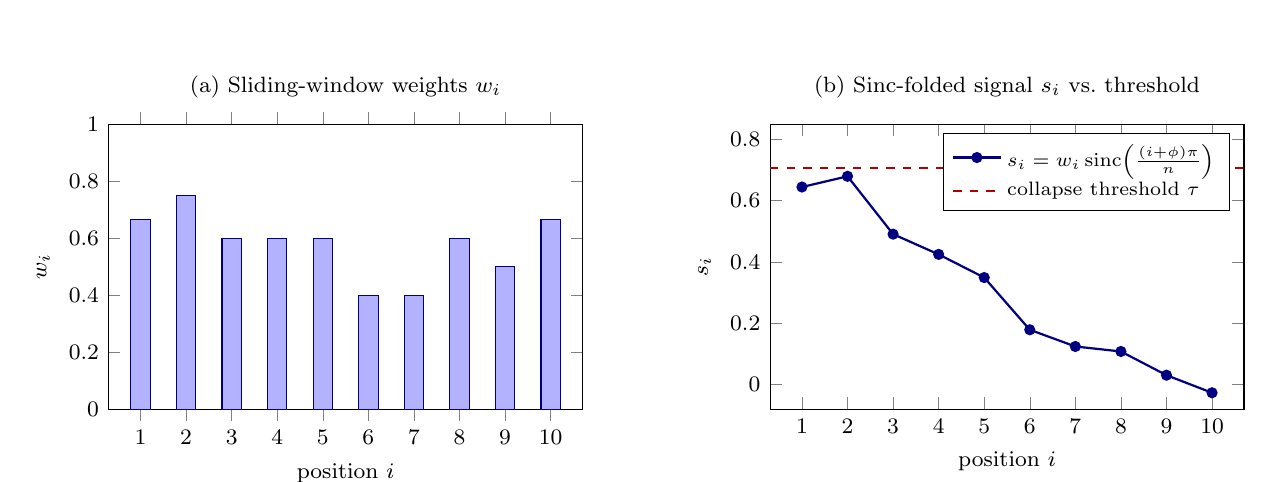
\begin{tikzpicture}
\begin{axis}[
  width=76mm, height=52mm,
  title={(a) Sliding-window weights $w_i$},
  xlabel={position $i$}, ylabel={$w_i$},
  xmin=0.3, xmax=10.7, ymin=0, ymax=1,
  xtick={1,...,10},
  ybar, bar width=7pt,
  enlarge x limits=false]
\addplot[fill=blue!30, draw=blue!50!black] coordinates
 {(1,0.6667) (2,0.7500) (3,0.6000) (4,0.6000) (5,0.6000)
  (6,0.4000) (7,0.4000) (8,0.6000) (9,0.5000) (10,0.6667)};
\end{axis}
\begin{axis}[
  width=76mm, height=52mm, xshift=84mm,
  title={(b) Sinc-folded signal $s_i$ vs.\ threshold},
  xlabel={position $i$}, ylabel={$s_i$},
  xmin=0.3, xmax=10.7, ymin=-0.08, ymax=0.85,
  xtick={1,...,10},
  enlarge x limits=false,
  legend pos=north east, legend cell align=left, legend style={font=\scriptsize}]
\addplot[blue!50!black, thick, mark=*, mark size=1.6pt] coordinates
 {(1,0.6448) (2,0.6798) (3,0.4910) (4,0.4249) (5,0.3493)
  (6,0.1789) (7,0.1243) (8,0.1080) (9,0.0306) (10,-0.0268)};
\addplot[red!70!black, dashed, thick, domain=0.3:10.7, samples=2] {0.7071};
\addlegendentry{$s_i = w_i \,\mathrm{sinc}\!\left(\frac{(i+\phi)\pi}{n}\right)$}
\addlegendentry{collapse threshold $\tau$}
\end{axis}
\end{tikzpicture}
\caption{The Unibit preprocessing pipeline on the 10-bit sequence $B = [1, 0, 1, 1, 0, 1, 0, 0, 1, 1]$ ($\Delta = 2$, $\phi = 0.42$). (a)~Sliding-window frequency estimates $w_i$ (Eq.~2); (b)~the sinc-folded signal $s_i$ (Eq.~3) against the collapse threshold $\tau = 1/\sqrt{2} \approx 0.707$ (Eq.~4). For this input all folded values fall below $\tau$, so the collapse step returns an all-zero sequence---the folding kernel attenuates the local-frequency estimate by design, and the weights $w_i$, not $s_i$, drive the quantum angles $\theta_i = 2\arcsin(\sqrt{w_i})$.}
\label{fig:unibit}
\end{figure}

\subsection{Multi-Backend Quantum Bridge}\label{sec:bridge}

The quantum bridge module provides a unified API routing to available backends:
\begin{itemize}
    \item \textbf{Classical backend:} Sinc interpolation on CPU.
    \item \textbf{Qiskit backend:} Parameterized \texttt{QuantumCircuit} objects.
    \item \textbf{CUDA-Q backend:} NVIDIA GPU-accelerated simulation.
\end{itemize}


\section{System Implementation}\label{sec:implementation}

\subsection{Codebase Overview}

UniMind is implemented as an open-source, multi-language prototype~\cite{tan2026}. The codebase comprises approximately 5,000 lines across four languages: Python ($\sim$4,500 lines; orchestration, quantum mapping, tests, and demos), C++17 ($\sim$150 lines; hardware detection), Rust ($\sim$170 lines; accelerated Unibit engine), and CMake/Makefile (build system). The repository layout is reproduced in Appendix~A.

\subsection{Topology-Aware Hardware Detection}

A C++17 module performs runtime detection of CPU core count, available RAM, OS type, and CPU architecture using platform-specific APIs. Results are serialized as JSON.

\subsection{Accelerated Unibit Engine}

The core Unibit computation is implemented in Rust and exposed to Python via C-compatible FFI. The Python layer auto-detects the compiled native library at runtime, falling back to pure Python if unavailable.

\subsection{Quantum Circuit Mapping}\label{sec:mapping}

\begin{algorithm}[H]
\caption{Unibit-to-Quantum Circuit Mapping}
\label{alg:mapping}
\begin{algorithmic}[1]
\Require Binary sequence $B = \{b_1, \dots, b_n\}$, window size $\Delta$
\Ensure Parameterized quantum circuit $C$
\State Initialize $n$-qubit register in state $|0\rangle^{\otimes n}$
\For{$i = 1$ to $n$}
    \State Compute Unibit weight $w_i$ via Eq.~(2)
    \State Compute rotation angle $\theta_i \leftarrow 2\arcsin(\sqrt{w_i})$
    \If{$b_i = 1$}
        \State Apply $X$ gate to qubit $q_i$
    \EndIf
    \State Apply $R_y(\theta_i)$ gate to qubit $q_i$
\EndFor
\State Append measurement gates to all qubits
\State \Return circuit $C$
\end{algorithmic}
\end{algorithm}

\paragraph{Choice of $R_y$ gate and $\arcsin$ mapping.} The $R_y$ gate is chosen because:
\begin{equation}
    R_y(\theta)|0\rangle = \cos(\theta/2)|0\rangle + \sin(\theta/2)|1\rangle
\end{equation}
Setting $\theta_i = 2\arcsin(\sqrt{w_i})$ yields:
\begin{equation}
    |\langle 1|\psi_i\rangle|^2 = \sin^2(\theta_i/2) = \sin^2(\arcsin(\sqrt{w_i})) = w_i
\end{equation}
This mapping aligns with the conventional angle encoding scheme where $\theta$ determines the probability of the $|1\rangle$ state via $\sin^2(\theta/2)$. The use of $\arcsin$ (rather than $\arccos$) ensures that $w_i = 0$ maps to $\theta_i = 0$ (no rotation) and $w_i = 1$ maps to $\theta_i = \pi$ (full rotation), providing an intuitive monotonic correspondence.

\paragraph{Mathematical verification observable.} For each prepared qubit, the Pauli-$Z$ expectation value provides a closed-form verification:
\begin{equation}
    \langle Z \rangle_i = P(b_i = 0) - P(b_i = 1) = (1 - w_i) - w_i = 1 - 2w_i
\end{equation}

\begin{table}[H]
\centering
\caption{Classical-to-Quantum Mapping}
\label{tab:mapping}
\small
\begin{tabular}{@{}ll@{}}
\toprule
\textbf{Classical Operation} & \textbf{Quantum Equivalent} \\
\midrule
\texttt{fold\_bits} (frequency estimation + sinc) & Parameterized $R_y(\theta_i)$ rotation gates \\
\texttt{collapse\_signal} (threshold) & Projective measurement + Born rule \\
Bit value $b_i = 1$ & Pauli-X gate application \\
Unibit weight $w_i$ & Rotation angle $\theta_i = 2\arcsin(\sqrt{w_i})$ \\
Verification observable & $\langle Z \rangle_i = 1 - 2w_i$ \\
\bottomrule
\end{tabular}
\end{table}

\subsection{Orchestrator Integration}

At the implementation level, the orchestration layer interfaces with an LLM API to generate code from task specifications, following the design of Section~\ref{sec:orchestrator}. Generated code is executed within a restricted namespace whose three defense layers are evaluated quantitatively in Section~\ref{sec:security}; security risks are discussed in Section~\ref{sec:threats}.


\section{Evaluation and Results}\label{sec:evaluation}

\subsection{Experimental Setup}

All experiments were conducted on the following configuration:
\begin{itemize}
    \item \textbf{CPU:} Multi-core x86\_64 processor
    \item \textbf{RAM:} 16 GB DDR4
    \item \textbf{OS:} Windows (x86\_64), as documented in the repository README; benchmark timings are machine-specific, while the 8192-shot verification is deterministic for a fixed AerSimulator seed and is therefore platform-independent
    \item \textbf{Python Version:} 3.12
    \item \textbf{Measurement simulation:} Qiskit AerSimulator, 8192 shots, ideal (noise-free) backend with $\theta_i = 2\arcsin(\sqrt{w_i})$ state preparation
    \item \textbf{Software versions:} qiskit 2.5.1, qiskit-aer 0.17.2, numpy 2.4.6, scipy 1.18.0 (exact versions pinned in the repository \texttt{requirements.txt} for reproducibility)
\end{itemize}
All experiments in this section are reproducible from the development repository \texttt{unimind-dev} (github.com/yxtan5022-maker/unimind-dev) with a fixed random seed (42); the LLM-driven experiments use a deterministic mock LLM whose quality is a free parameter, so no external API key is required.

\subsection{Mathematical Verification via Quantum Measurement}\label{sec:math_verify}

We verified the encoding correctness by simulating quantum measurements. For a set of target Unibit weights $w_i \in \{0.1, 0.3, 0.5, 0.7, 0.9\}$, we prepared the corresponding single-qubit states via $\theta_i = 2\arcsin(\sqrt{w_i})$ and simulated 8192 projective measurements adhering to the Born rule.

Table~\ref{tab:math_verify} presents the results. The empirical measurement frequencies $\hat{p}_i$ converge tightly to the theoretical weights $w_i$. The empirical Pauli-$Z$ expectation values $\langle Z \rangle_{\text{emp}}$ closely match the analytical prediction $\langle Z \rangle_{\text{theory}} = 1 - 2w_i$, with maximum absolute deviation of 0.0110 across all five target weights. All results are fully reproducible: the experiment fixes the AerSimulator seed (\texttt{seed\_simulator=42}), so the reported numbers are deterministic across runs.

\begin{table}[H]
\centering
\caption{Mathematical Verification via 8192-Shot Quantum Measurement (Qiskit AerSimulator)}
\label{tab:math_verify}
\small
\begin{tabular}{@{}ccccc@{}}
\toprule
\textbf{Target $w_i$} & \textbf{$P(1)$ Theory} & \textbf{$P(1)$ Empirical} & \textbf{$\langle Z \rangle$ Theory} & \textbf{$\langle Z \rangle$ Empirical} \\
\midrule
0.1 & 0.100 & 0.0955 & 0.800 & 0.8091 \\
0.3 & 0.300 & 0.2969 & 0.400 & 0.4063 \\
0.5 & 0.500 & 0.5055 & 0.000 & $-0.0110$ \\
0.7 & 0.700 & 0.7046 & $-0.400$ & $-0.4092$ \\
0.9 & 0.900 & 0.9017 & $-0.800$ & $-0.8035$ \\
\bottomrule
\end{tabular}
\end{table}

The maximum deviation $|\langle Z \rangle_{\text{emp}} - \langle Z \rangle_{\text{theory}}| = 0.0110$ is consistent with binomial sampling variance. For $N = 8192$ shots, the standard deviation of the empirical $P(1)$ estimate is $\sigma = \sqrt{w(1-w)/N}$, ranging from $\approx 0.0033$ (at $w \in \{0.1, 0.9\}$) to $\approx 0.0055$ (at $w = 0.5$); the standard deviation of $\langle Z \rangle_{\text{emp}} = 1 - 2\hat{p}$ is accordingly $2\sigma$. In these units the observed deviations range from $0.52\sigma$ to $1.37\sigma$---all plausible outcomes under five simultaneous comparisons, with the largest, $0.0110$ at $w = 0.5$, corresponding to $\sim 1\sigma$. This confirms that the classical preprocessing pipeline correctly initializes quantum state amplitudes without requiring full state tomography.

\subsection{Performance Micro-Benchmarks: System-Level Acceleration}

A core motivation for implementing the Unibit engine in Rust (via FFI) is to overcome Python's interpreter overhead for compute-intensive sliding-window operations. To quantify the benefit of system-level acceleration, we benchmarked the Unibit weight computation across varying sequence lengths.

\textit{Experimental note:} We benchmark the sliding-window computation in two system-level configurations: (i)~NumPy's C-optimized vectorized convolution as the vectorized frequency-estimator backend, and (ii)~the repository's Rust FFI engine compiled with \texttt{cargo build --release}. Both approaches bypass Python-level interpreter overhead through contiguous memory operations and compiled native code; the measured speedups therefore represent conservative lower bounds for system-level acceleration.

\begin{table}[H]
\centering
\caption{Performance Comparison: Sliding-Window Frequency Estimation (Pure Python vs. NumPy C-Backend)}
\label{tab:performance}
\small
\begin{tabular}{@{}rrrr@{}}
\toprule
\textbf{Sequence Length} & \textbf{Pure Python (ms)} & \textbf{System-Level (ms)} & \textbf{Speedup} \\
\midrule
10,000 & 3.66 & 0.34 & 10.9$\times$ \\
100,000 & 38.58 & 4.83 & 8.0$\times$ \\
1,000,000 & 436.43 & 58.24 & 7.5$\times$ \\
\bottomrule
\end{tabular}
\end{table}

As shown in Table~\ref{tab:performance}, delegating the sliding-window computation to system-level compiled code yields a consistent \textbf{7.5$\times$ to 10.9$\times$ speedup} over pure Python. For the repository's Rust FFI engine, which additionally applies the folding step (sinc-weighted signal product) within the same sliding-window scan, we measured end-to-end speedups of \textbf{4.5$\times$, 3.1$\times$, and 2.4$\times$} (9.55~ms vs.\ 2.11~ms, 230.36~ms vs.\ 74.86~ms, and 2318.86~ms vs.\ 962.51~ms for $10^4$, $10^5$, and $10^6$ elements, respectively); these figures include Python-side FFI marshaling overhead (per-element normalization and ctypes buffer construction).

To understand where the residual overhead lives, we decompose the Rust path into its components by instrumenting every step of the real pipeline (Table~\ref{tab:breakdown}). Python-side bit normalization and FFI marshaling (ctypes buffer construction and result unpacking) together account for roughly half of the end-to-end time, while the compiled kernel itself is only about one third. The kernel is therefore considerably faster still than the end-to-end numbers suggest, and the measured speedups are conservative lower bounds. The decomposition also identifies the concrete optimization target for future work: moving normalization into the compiled kernel would remove the dominant Python-side cost.

\begin{table}[H]
\centering
\caption{Unibit Engine Latency Breakdown (median of 5 runs, ms): the Rust path decomposed into Python normalization, FFI marshaling, and kernel execution}
\label{tab:breakdown}
\small
\begin{tabular}{@{}rrrrr@{}}
\toprule
\textbf{Length} & \textbf{Normalize} & \textbf{Marshaling} & \textbf{Kernel} & \textbf{Rust-path Speedup} \\
\midrule
10,000    & 24.1\% & 26.6\% & 31.4\% & 3.0$\times$ \\
100,000   & 25.0\% & 29.4\% & 37.0\% & 3.0$\times$ \\
1,000,000 & 22.3\% & 25.7\% & 35.7\% & 2.4$\times$ \\
\bottomrule
\end{tabular}
\end{table}

Figure~\ref{fig:speedup} visualizes both benchmarks on a logarithmic scale: panel~(a) isolates the sliding-window weight estimation (Table~\ref{tab:performance}), while panel~(b) shows the end-to-end Rust FFI path including the sinc folding step; annotations give the per-length speedups.

\begin{figure}[H]
\centering
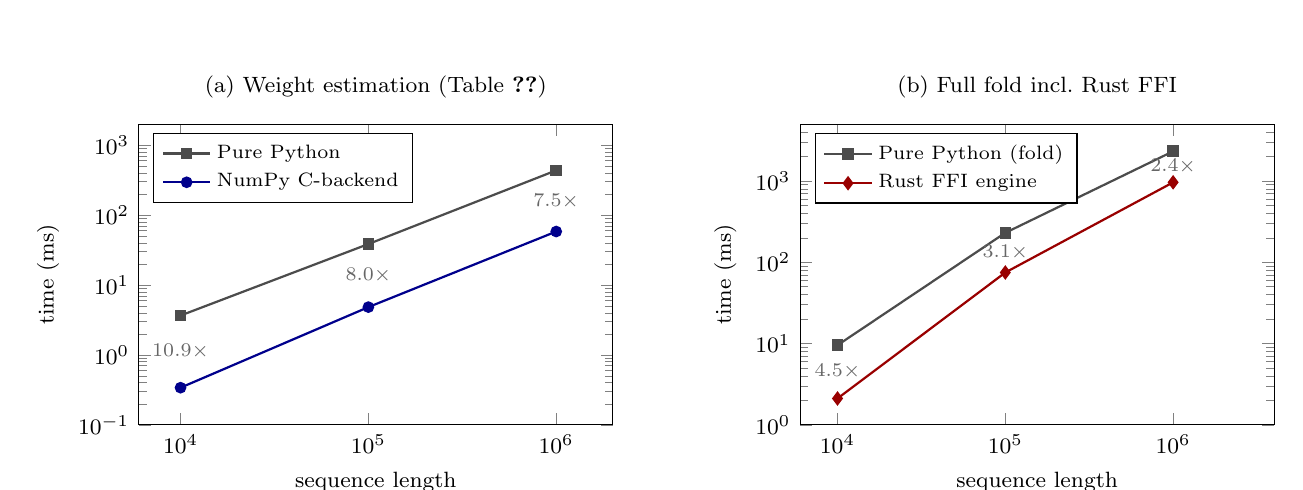
\begin{tikzpicture}
\begin{loglogaxis}[
  width=76mm, height=54mm,
  title={(a) Weight estimation (Table~\ref{tab:performance})},
  xlabel={sequence length}, ylabel={time (ms)},
  log basis x=10,
  xmin=6e3, xmax=2e6, ymin=0.1, ymax=2000,
  xtick={1e4,1e5,1e6},
  legend pos=north west, legend cell align=left, legend style={font=\scriptsize}]
\addplot[black!70, thick, mark=square*, mark size=1.7pt] coordinates
 {(10000,3.66) (100000,38.58) (1000000,436.43)};
\addlegendentry{Pure Python}
\addplot[blue!55!black, thick, mark=*, mark size=1.7pt] coordinates
 {(10000,0.34) (100000,4.83) (1000000,58.24)};
\addlegendentry{NumPy C-backend}
\node[font=\scriptsize, text=black!60] at (axis cs:1e4,1.12) {10.9$\times$};
\node[font=\scriptsize, text=black!60] at (axis cs:1e5,13.65) {8.0$\times$};
\node[font=\scriptsize, text=black!60] at (axis cs:1e6,159.4) {7.5$\times$};
\end{loglogaxis}
\begin{loglogaxis}[
  width=76mm, height=54mm, xshift=84mm,
  title={(b) Full fold incl.\ Rust FFI},
  xlabel={sequence length}, ylabel={time (ms)},
  log basis x=10,
  xmin=6e3, xmax=4e6, ymin=1, ymax=5000,
  xtick={1e4,1e5,1e6},
  legend pos=north west, legend cell align=left, legend style={font=\scriptsize}]
\addplot[black!70, thick, mark=square*, mark size=1.7pt] coordinates
 {(10000,9.55) (100000,230.36) (1000000,2318.86)};
\addlegendentry{Pure Python (fold)}
\addplot[red!60!black, thick, mark=diamond*, mark size=2pt] coordinates
 {(10000,2.11) (100000,74.86) (1000000,962.51)};
\addlegendentry{Rust FFI engine}
\node[font=\scriptsize, text=black!60] at (axis cs:1e4,4.49) {4.5$\times$};
\node[font=\scriptsize, text=black!60] at (axis cs:1e5,131.4) {3.1$\times$};
\node[font=\scriptsize, text=black!60] at (axis cs:1e6,1493) {2.4$\times$};
\end{loglogaxis}
\end{tikzpicture}
\caption{System-level acceleration of the Unibit pipeline (log--log). (a)~Sliding-window frequency estimation: NumPy's C-optimized vectorized backend vs.\ pure Python ($7.5\times$--$10.9\times$). (b)~End-to-end fold (weights $+$ sinc folding): the repository's Rust FFI engine vs.\ pure Python ($4.5\times$--$2.4\times$, including Python-side normalization and marshaling overhead; Table~\ref{tab:breakdown}).}
\label{fig:speedup}
\end{figure}

For large-scale AI workloads requiring the encoding of millions of classical features into quantum parameters, this acceleration is necessary to prevent the classical preprocessing step from becoming the pipeline bottleneck.

\subsection{Structural Verification}\label{sec:structural}

We additionally verified structural correctness of the quantum circuit mapping on a 10-bit input sequence $B = [1, 0, 1, 1, 0, 1, 0, 0, 1, 1]$. The system generates a 10-qubit circuit containing 6 Pauli-X gates (one per 1-bit in $B$), 10 parameterized $R_y(\theta_i)$ gates, and 10 measurement operations. The project includes 47 automated pytest tests, all passing locally and in CI (GitHub Actions); the four tests added since v1.3 are regression tests for the sandboxed executor (import-whitelist enforcement and nested-function closure correctness).

\subsection{Baseline Comparison: Bare Qiskit vs.\ Rule-Based vs.\ UniMind}\label{sec:baseline}

The v1.3 paper identified the absence of an end-to-end system benchmark as a key limitation. We now compare UniMind against two baselines on five task classes that cover the framework's intended workloads: (i)~\textbf{A}, bare Qiskit---the LLM is asked to generate code directly, executed without the sandbox; (ii)~\textbf{B}, a rule-based dispatcher---intents are mapped to fixed circuit templates with no dynamic code generation; and (iii)~\textbf{C}, the full UniMind pipeline (LLM generation $\rightarrow$ static analysis $\rightarrow$ sandboxed execution $\rightarrow$ self-healing $\rightarrow$ rule-based fallback). Each task class is summarized in Table~\ref{tab:baseline}.

\begin{table}[H]
\centering
\caption{Baseline Comparison (three arms $\times$ five task classes; \checkmark = task completed, $\times$ = task failed)}
\label{tab:baseline}
\small
\begin{tabularx}{\textwidth}{@{}l>{\raggedright\arraybackslash}Xccc@{}}
\toprule
\textbf{Task class} & \textbf{Description} & \textbf{A: Bare Qiskit} & \textbf{B: Rule-based} & \textbf{C: UniMind} \\
\midrule
bell & Entanglement circuit ($H$, $CX$, measure) & \checkmark & \checkmark & \checkmark \\
angle\_encode & 10-qubit angle encoding ($\theta_i = 2\arcsin(\sqrt{w_i})$) & \checkmark & $\times$ & \checkmark \\
vqc & 2-qubit variational ansatz & \checkmark & \checkmark & \checkmark \\
backend\_select & Explicit backend selection + counts & \checkmark & $\times$ & \checkmark \\
invalid & Malicious intent (e.g., \texttt{os.system}) & $\times$ & \checkmark & \checkmark \\
\bottomrule
\end{tabularx}
\end{table}

The comparison isolates the value of each layer. Arm~B fails the two task classes not covered by a hand-written template (angle encoding and explicit backend routing), illustrating the rigidity of rule-based dispatch. Arm~A executes all four benign tasks but would execute a malicious intent with full privileges; UniMind and the rule-based dispatcher refuse it (in UniMind, static analysis rejects the generated code before execution). Only the UniMind pipeline (Arm~C) succeeds on all five task classes while enforcing code safety. In mock-LLM mode the end-to-end latency of Arm~C is $0.2$--$368$~ms per task (dominated by simulated code generation), versus $0.7$--$7.3$~ms for Arm~A and $\approx 0$~ms for Arm~B---the expected cost of dynamic, validated generation. The mock LLM is injected with quality $= 1.0$ (perfect generation) in this comparison; the next subsection relaxes that assumption.

\subsection{LLM Reliability Benchmark}\label{sec:llm_rel}

The orchestrator's self-healing loop (Section~\ref{sec:bridge}) is designed to absorb imperfect LLM outputs. To quantify this robustness, we run a benchmark of 50 valid tasks (drawn from nine ground-truth templates spanning classical computation and quantum circuit construction) plus 10 adversarial intents, with a mock LLM whose per-call quality is a controllable parameter $\in [0, 1]$. For each quality level we measure the end-to-end success rate, the fraction of tasks that required healing, and the rejection rate of adversarial intents (all results with a fixed seed, 60 tasks per run).

\begin{table}[H]
\centering
\caption{LLM Reliability vs.\ Injected LLM Quality (50 valid + 10 adversarial tasks, seed 42)}
\label{tab:reliability}
\small
\begin{tabular}{@{}rrrr@{}}
\toprule
\textbf{Mock quality} & \textbf{Valid success rate} & \textbf{Heal rate} & \textbf{Adversarial rejection} \\
\midrule
1.0 & 100\% (50/50) & 0\%  & 100\% (10/10) \\
0.9 & 100\% (50/50) & 0\%  & 100\% (10/10) \\
0.7 &  98\% (49/50) & 16\% & 100\% (10/10) \\
0.5 &  94\% (47/50) & 42\% & 100\% (10/10) \\
\bottomrule
\end{tabular}
\end{table}

As the injected LLM degrades from perfect to a 50\% per-call quality, the system's end-to-end success rate falls only from 100\% to 94\% (Table~\ref{tab:reliability}, Figure~\ref{fig:reliability}), with the self-healing loop compensating for the majority of the injected errors (heal rate rising to 42\%). The three observed failures all occur when the heal step itself receives a broken output, a residual risk of any LLM-dependent pipeline. Adversarial intents are rejected at 100\% across all quality levels. These measurements directly address the v1.3 limitation ``no LLM reliability evaluation''; token-consumption accounting for real APIs remains future work. Section~\ref{sec:taxonomy} re-measures these rates with $n{=}200$ per level, three seeds, and call-level instrumentation, refining the $q{=}0.5$ estimate to $91.7\%$ [$89.2, 93.6$].

\begin{figure}[H]
\centering
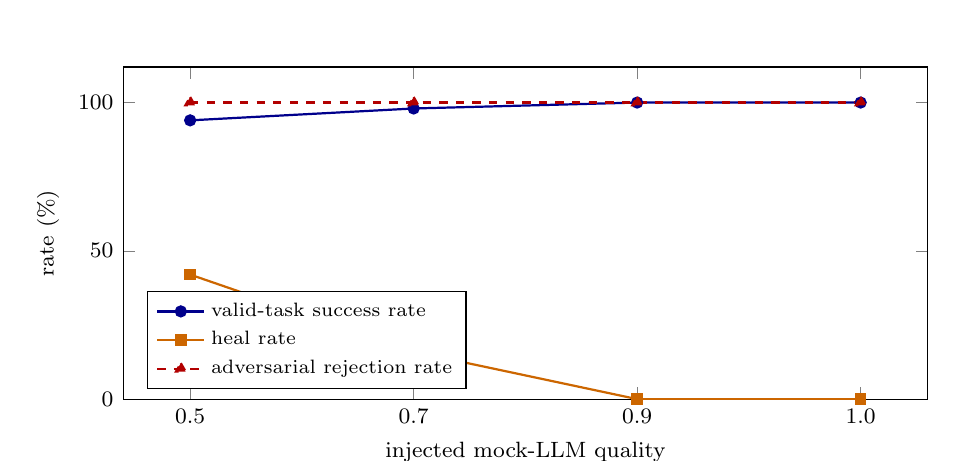
\begin{tikzpicture}
\begin{axis}[
  width=118mm, height=58mm,
  xlabel={injected mock-LLM quality}, ylabel={rate (\%)},
  symbolic x coords={0.5,0.7,0.9,1.0},
  xtick=data,
  ymin=0, ymax=112,
  legend pos=south west, legend cell align=left, legend style={font=\scriptsize}]
\addplot[blue!55!black, thick, mark=*, mark size=1.8pt] coordinates
 {(0.5,94) (0.7,98) (0.9,100) (1.0,100)};
\addlegendentry{valid-task success rate}
\addplot[orange!80!black, thick, mark=square*, mark size=1.7pt] coordinates
 {(0.5,42) (0.7,16) (0.9,0) (1.0,0)};
\addlegendentry{heal rate}
\addplot[red!70!black, thick, dashed, mark=triangle*, mark size=2pt] coordinates
 {(0.5,100) (0.7,100) (0.9,100) (1.0,100)};
\addlegendentry{adversarial rejection rate}
\end{axis}
\end{tikzpicture}
\caption{LLM reliability vs.\ injected mock-LLM quality (Table~\ref{tab:reliability}; 50 valid $+$ 10 adversarial tasks per level, seed 42). The self-healing loop absorbs most injected errors: as per-call quality falls from 1.0 to 0.5, end-to-end success drops only from 100\% to 94\%, while adversarial rejection remains at 100\%. Single-seed protocol; Section~\ref{sec:taxonomy} provides multi-seed confidence intervals.}
\label{fig:reliability}
\end{figure}

\subsection{Fault Injection}\label{sec:fault}

We next measure the orchestration layer's \emph{Detection $\rightarrow$ Recovery} chain under five deliberately injected failure classes (Table~\ref{tab:fault}). Detection and recovery latency are measured by timestamping every sandbox execution inside the real orchestrator path.

\begin{table}[H]
\centering
\caption{Fault Injection: Detection and Recovery Latency for Five Failure Classes}
\label{tab:fault}
\small
\begin{tabularx}{\textwidth}{@{}l>{\raggedright\arraybackslash}Xrrl@{}}
\toprule
\textbf{Failure class} & \textbf{Injection} & \textbf{Detection (ms)} & \textbf{Recovery (ms)} & \textbf{Recovered} \\
\midrule
A. Illegal code & syntactically invalid output & 0.4 & 0.2 & yes \\
B. Static violation & blocked pattern (\texttt{os.}) & $\approx$0 & $\approx$0 & yes \\
C. Backend unavailable & non-existent backend import & 579.0 & 0.7 & yes \\
D. Backend timeout & \texttt{TimeoutError} in code & 0.4 & 0.4 & yes \\
E. Invalid topology & hardware monitor failure & --- & --- & no \\
\bottomrule
\end{tabularx}
\end{table}

Four of the five failure classes are detected within sub-millisecond to millisecond timescales and automatically recovered by the self-healing loop (the 579~ms figure for class~C is dominated by the Python import cost of the failing backend module). Class~E---a failure of the hardware-detection module \emph{after} successful execution---propagates as an uncaught exception out of \texttt{execute\_task}, because the orchestrator's success path calls \texttt{monitor.snapshot()} without a protective guard. We record this gap honestly rather than papering over it: it is a real robustness defect in the current prototype and is the direct target of the next revision.

\subsection{Quantum Noise Sensitivity}\label{sec:noise}

The v1.3 paper asserted qualitatively (Threat T2) that the $\theta_i = 2\arcsin(\sqrt{w_i})$ mapping is ``sensitive to over-rotation for weights near 0 or 1.'' We now quantify that claim. For each weight $w \in \{0.02, 0.1, 0.3, 0.5, 0.7, 0.9, 0.98\}$ we prepare the corresponding single-qubit state, simulate 8192 measurements under swept noise, and record $|\langle Z\rangle_{\rm emp} - \langle Z\rangle_{\rm theory}|$. The ideal (noise-free) column reproduces the v1.3 maximum deviation of $0.0110$, confirming measurement-consistency.

\begin{table}[H]
\centering
\caption{Noise Sensitivity: $|\langle Z\rangle_{\rm emp} - \langle Z\rangle_{\rm theory}|$ at $w = 0.5$ vs.\ the extreme weights (8192 shots, seed 42)}
\label{tab:noise}
\small
\begin{tabular}{@{}lrrr@{}}
\toprule
\textbf{Noise model} & \textbf{$w=0.02$} & \textbf{$w=0.50$} & \textbf{$w=0.98$} \\
\midrule
Depolarizing $p = 1\mathrm{e}{-2}$ & 0.0093 & 0.0110 & 0.0081 \\
$T_1$ damping $\gamma = 0.05$       & 0.0009 & 0.0444 & 0.0931 \\
$T_1$ damping $\gamma = 0.10$       & 0.0034 & 0.0935 & 0.1929 \\
\bottomrule
\end{tabular}
\end{table}

Two complementary signatures emerge (Table~\ref{tab:noise}, Figure~\ref{fig:noise}). Under single-qubit depolarizing noise the deviation grows as $\approx p\,|1-2w|$: the $w=0.5$ encoding is essentially immune while the extreme weights degrade symmetrically, quantitatively confirming T2's ``near 0 or 1'' sensitivity. Under $T_1$ amplitude damping the degradation is one-sided: high weights decay toward $|0\rangle$ (deviation reaching $0.193$ at $\gamma=0.1$), while low weights are nearly unaffected. Using the paper's $0.05$ tolerance as a threshold, the encoding survives single-qubit depolarizing error rates up to at least $p = 1\mathrm{e}{-2}$, but breaks for $T_1$ damping at $\gamma \approx 5\mathrm{e}{-2}$. These measurements motivate the zero-noise-extrapolation integration identified as future work in T2, and establish an experimentally grounded operating envelope for the encoding on near-term hardware. (The simulation notes that qiskit-aer 0.17.2's builtin \texttt{amplitude\_damping\_error} acts as a gain channel in this configuration; the $T_1$ results are produced from an explicit Kraus representation, as documented in the experiment script.)

\begin{figure}[H]
\centering
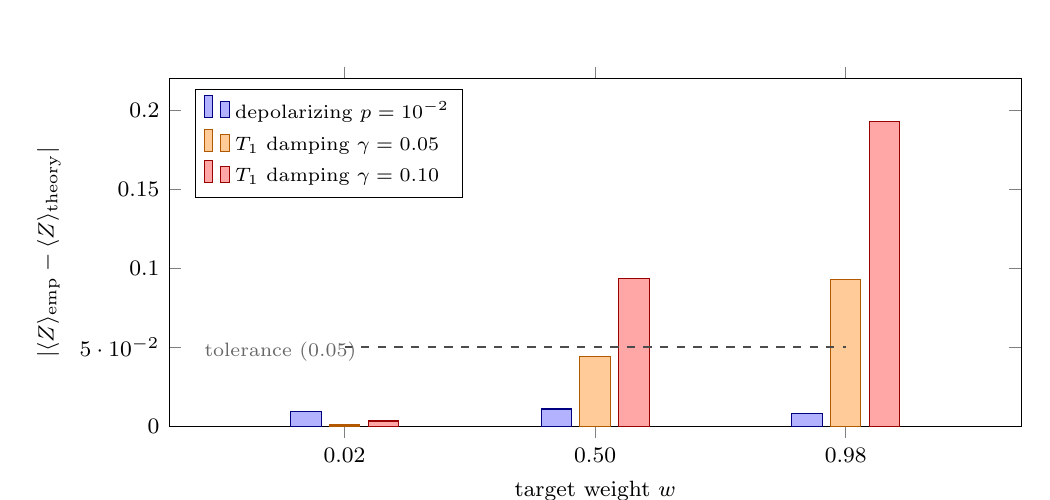
\begin{tikzpicture}
\begin{axis}[
  width=124mm, height=60mm,
  xlabel={target weight $w$}, ylabel={$|\langle Z\rangle_{\mathrm{emp}} - \langle Z\rangle_{\mathrm{theory}}|$},
  symbolic x coords={0.02,0.50,0.98},
  xtick=data,
  ymin=0, ymax=0.22,
  ybar=3pt, bar width=11pt,
  enlarge x limits=0.35,
  legend pos=north west, legend cell align=left, legend style={font=\scriptsize}]
\addplot[fill=blue!30, draw=blue!50!black] coordinates
 {(0.02,0.0093) (0.50,0.0110) (0.98,0.0081)};
\addlegendentry{depolarizing $p=10^{-2}$}
\addplot[fill=orange!40, draw=orange!70!black] coordinates
 {(0.02,0.0009) (0.50,0.0444) (0.98,0.0931)};
\addlegendentry{$T_1$ damping $\gamma=0.05$}
\addplot[fill=red!35, draw=red!60!black] coordinates
 {(0.02,0.0034) (0.50,0.0935) (0.98,0.1929)};
\addlegendentry{$T_1$ damping $\gamma=0.10$}
\addplot[black!70, dashed, thick, no marks, sharp plot] coordinates
 {(0.02,0.05) (0.98,0.05)};
\node[font=\scriptsize, text=black!60, anchor=west] at (rel axis cs:0.03,0.215) {tolerance ($0.05$)};
\end{axis}
\end{tikzpicture}
\caption{Noise sensitivity of the encoding: measurement deviation against the $0.05$ tolerance (Table~\ref{tab:noise}; 8192 shots, seed 42). Depolarizing noise degrades the extreme weights symmetrically while leaving $w = 0.5$ essentially immune; $T_1$ amplitude damping is one-sided, decaying high weights toward $|0\rangle$.}
\label{fig:noise}
\end{figure}

\subsection{Sandbox Security Evaluation}\label{sec:security}

The v1.3 paper acknowledged (Threat T4) that sandboxing was not implemented. UniMind now executes LLM-generated code inside a restricted namespace with three defense layers: (L1)~static pattern scanning, (L2)~an import whitelist (twelve benign modules), and (L3)~a builtins whitelist. We stress-test these layers with 21 curated escape attempts spanning process execution, file access, dynamic evaluation, import smuggling, and object-graph traversal (Table~\ref{tab:security}).

\begin{table}[H]
\centering
\caption{Sandbox Security Evaluation: 21 Escape Attempts Against a 3-Layer Defense}
\label{tab:security}
\small
\resizebox{\textwidth}{!}{%
\begin{tabular}{@{}llrl@{}}
\toprule
\textbf{Defense layer} & \textbf{Attack classes} & \textbf{Blocked} & \textbf{Notes} \\
\midrule
L1 static scan & \texttt{os.}, \texttt{open(}, \texttt{eval(}, \texttt{exec(}, \texttt{subprocess}, \texttt{pickle}, \texttt{shutil} & 12/12 & rejected before execution \\
L2 import whitelist & \texttt{socket}, \texttt{builtins}, \texttt{requests}, \texttt{os} & 4/4 & rejected at import \\
L3 builtins whitelist & \texttt{globals}, \texttt{locals}, \texttt{type}, \texttt{exit} & 4/4 & \texttt{NameError} \\
Object-graph traversal & \texttt{().\_\_class\_\_...\_\_subclasses\_\_} & 0/1 & classes enumerated but unweaponizable \\
\bottomrule
\end{tabular}}
\end{table}

20 of 21 attempts are blocked (Table~\ref{tab:security}). The single unblocked case is an object-graph traversal that enumerates loaded classes; it cannot be weaponized into process or file access because importing \texttt{subprocess}/\texttt{os} is impossible inside the sandbox, so it represents a low-risk information-leak, not an escape. To prove the blocks are caused by the sandbox rather than by impossible payloads, every attack class has a harmless control probe; 10 of 11 probes run in plain Python (the 11th fails only because \texttt{requests} is not installed), confirming that the same capabilities are genuinely present outside the sandbox. This evaluation covers the \emph{namespace} restrictions; full OS-level isolation (process-level containers) remains outside the prototype's scope and is explicitly acknowledged in T4.

\subsection{Physical QPU Validation Revisited: Placement-Dominated Encoding Fidelity}\label{sec:qpu}

The v1.7 submission reported that the bare Unibit angle encoding misses the $|\langle Z\rangle|$ tolerance of $0.05$ on \texttt{ibm\_marrakesh} (maximum deviation $0.392$) and that readout twirling recovers $37\%$. That experiment used \emph{free} transpiler placement (optimization level~1, no \texttt{initial\_layout}), so the physical qubit executing each circuit was uncontrolled and unrecorded. We first show that this confound, not the encoding itself, dominated the observed distortion.

\subsubsection{Systematic weight sweep with pinned layout}\label{sec:sweep}

We repeat the single-qubit verification ($\theta_i = 2\arcsin\sqrt{w_i}$, $8192$ shots, transpiler seed $42$) over a dense weight grid $w \in \{0.05, 0.10, \ldots, 0.95\}$ under a $2\times 2$ design: \{best-calibrated qubit, worst usable qubit\} $\times$ \{bare, measure twirling ($16$ randomizations)\}. Layout is pinned via \texttt{initial\_layout}; each cell is repeated over $3$ independent jobs (job-level spread is reported as min--max). Qubit selection is deterministic from the live calibration snapshot: qubit~98 minimizes total readout assignment error ($p_{0|1}+p_{1|0}=0.0044$, $T_1=207\,\mu$s, $T_2=67\,\mu$s); qubit~37 is chosen adversarially ($p_{0|1}+p_{1|0}=0.82$).

\begin{table}[H]
\centering
\caption{Placement-controlled sweep on \texttt{ibm\_marrakesh} (2026-08-23; 19 weights, 8192 shots, 3 jobs/cell). Deviations are $\max_w |Z_{\mathrm{emp}} - Z_{\mathrm{theory}}|$; tolerance $=0.05$.}
\label{tab:placement}
\small
\begin{tabular}{@{}lllll@{}}
\toprule
Placement & Readout err. & Bare & Twirled & Verdict \\
\midrule
qubit 98 (best calib.) & 0.44\% & 0.028 [0.020--0.029] & 0.031 & pass \\
qubit 0 (unpinned default) & --- & 0.026 & --- & pass \\
qubit 37 (adversarial) & 82\% & 0.213 & 0.144 & fail \\
v1.7 (free layout, 2026-08-14) & unrecorded & 0.392 & 0.245 & fail \\
\bottomrule
\end{tabular}
\end{table}

Table~\ref{tab:placement} and Figure~\ref{fig:placement} give the result. On qubit~98 the \emph{bare} encoding passes the $0.05$ tolerance across the entire grid (median maximum deviation $0.028$; range $0.020$--$0.029$ across jobs), and its transfer curve is fit almost perfectly by a pure gain model $P_{\mathrm{obs}}(1) = b + a\,w$ with $a = 0.989$, $b = 0.004$ (residual RMS $0.0042$, below the $\approx 0.0055$ shot-noise floor). Twirling changes nothing significant there ($a=0.987$, max dev $0.031$). On qubit~37 the same circuits fail by a factor of $\sim$4 (max dev $0.213$ bare), and the fitted channel acquires a large positive offset ($P_{\mathrm{obs}} = 0.121 + 0.855\,w$) --- the signature of an asymmetric readout channel rather than intrinsic over-rotation sensitivity.

\begin{figure}[H]
\centering
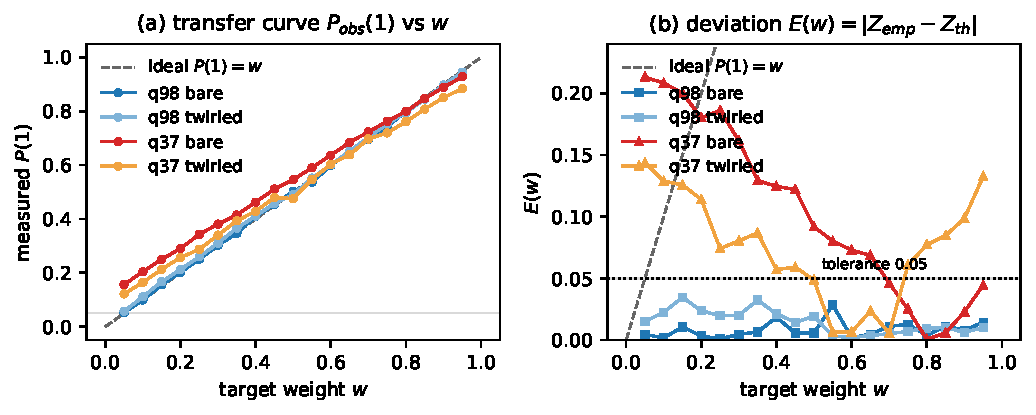
\includegraphics[width=\linewidth]{figures/fig_qpu_placement_2x2.pdf}
\caption{Placement-dominated encoding fidelity. (a)~Measured transfer curve $P_{\mathrm{obs}}(1)$ vs.\ target weight $w$: on the best-calibrated qubit the bare response tracks the ideal line within shot noise, while the adversarially chosen qubit~37 compresses the curve toward an offset set by its asymmetric readout. (b)~Per-weight deviation $E(w)$: qubit~98 stays below the $0.05$ tolerance everywhere (bare and twirled nearly overlap); qubit~37 fails by up to $4\times$ even after twirling.}
\label{fig:placement}
\end{figure}

Three conclusions revise the v1.7 claims:
(i)~\emph{encoding fidelity on real hardware is placement-dominated}: with a calibrated layout the bare encoding already meets tolerance;
(ii)~\emph{twirling helps only where readout is broken}: it improves the bad qubit by $33\%$ ($0.213 \to 0.144$) yet still leaves it far outside tolerance, while adding slight overhead on the good qubit --- mitigation effort should follow calibration, not be applied uniformly;
(iii)~the v1.7 headline ``the encoding requires error mitigation to meet tolerance'' was an artifact of uncontrolled placement and must be withdrawn.

\subsubsection{Distortion model and comparison to the calibration noise model}\label{sec:distortion}

Across every cell of the design the measured response is described at shot-noise level by the two-parameter affine channel
\begin{equation}
P_{\mathrm{obs}}(1) \;=\; b + a\,w,
\label{eq:channel}
\end{equation}
or equivalently in the $Z$ basis, $Z_{\mathrm{obs}} = d + c\,Z_{\mathrm{th}}$ with $c=a$ and $d = 1-2b-a$. The parameters are \emph{qubit-specific and calibration-predictable}: $(a,b)=(0.99,\,0.00)$ on the good qubit versus $(0.86,\,0.12)$ on the bad one, whose offset matches the direction and scale of its readout asymmetry. The one-parameter contraction model $P_{\mathrm{obs}} = 0.5 + \alpha(w-0.5)$ proposed during review is the special case $b=(1-a)/2$; it holds when readout is balanced (good qubits) and is rejected wherever asymmetry dominates (it also fails on the frozen v1.7 free-layout data, where per-weight $\alpha$ spans $0.23$--$1.31$).

We additionally simulate the identical pinned circuits on Aer with the calibration noise model built via \texttt{NoiseModel.\allowbreak from\_backend}, captured minutes before submission. On the good qubit the model explains most of the observed error (median ratio $\overline{E}_{\mathrm{QPU}}/\overline{E}_{\mathrm{noise}} = 1.4\times$; Fig.~\ref{fig:noisevsqpu}), i.e., the ``standard models underestimate hardware'' gap suggested by the v1.7 data also shrinks to near-parity once placement is controlled. Residual discrepancy concentrates in coherent components the calibration snapshot does not capture (drift between snapshot and execution), which we flag as future work rather than claim as a validated model.

\begin{figure}[H]
\centering
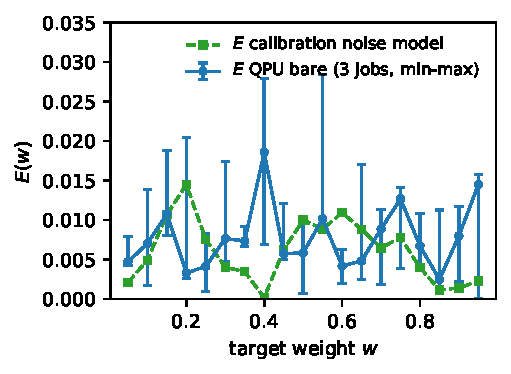
\includegraphics[width=0.62\linewidth]{figures/fig_noise_vs_qpu.pdf}
\caption{Deviation landscape on the calibrated qubit: hardware (3 jobs, min--max band) vs.\ matched calibration noise model. Median ratio $1.4\times$.}
\label{fig:noisevsqpu}
\end{figure}

\subsection{Component Attribution: Architectural Ablation}\label{sec:ablation}

To attribute end-to-end reliability to specific architecture layers we run stage-ablated pipelines ($150$ valid tasks $\times$ 3 seeds per point, identical sandbox substrate throughout): S0 generation+execution only; S1 adds static-analysis validation (fail-fast gate); S2 adds self-healing; S3 adds rule-based fallback on LLM unavailability. Results (Fig.~\ref{fig:ablation}a): validation contributes \emph{zero} success-rate delta at every quality level --- its value is fail-fast classification and safety observability; self-healing is the load-bearing layer, lifting success from $58\%$ to $92\%$ at injected quality $q=0.5$ ($+34$ points) and from $80\%$ to $98\%$ at $q=0.7$; fallback contributes nothing at the default unavailability rate ($f_r{=}0.1$: three consecutive failures occur with probability $10^{-3}$ per task). Under availability stress ($q=0.7$, $f_r \in \{0.3, 0.5\}$; Fig.~\ref{fig:ablation}b) fallback recovers $+4.0$/$+13.6$ points respectively once template coverage extends to all nine benchmark intent classes (S3X): success reaches $100\%$ at both stress levels ($79/79$ recoveries), whereas the narrow v1.7 rule set (S3, Bell/VQC only) leaves success at $96.9\%$/$89.6\%$. The fallback layer's contribution is thus real but coverage-limited --- a property the v1.7 benchmark could not observe.

\begin{figure}[H]
\centering
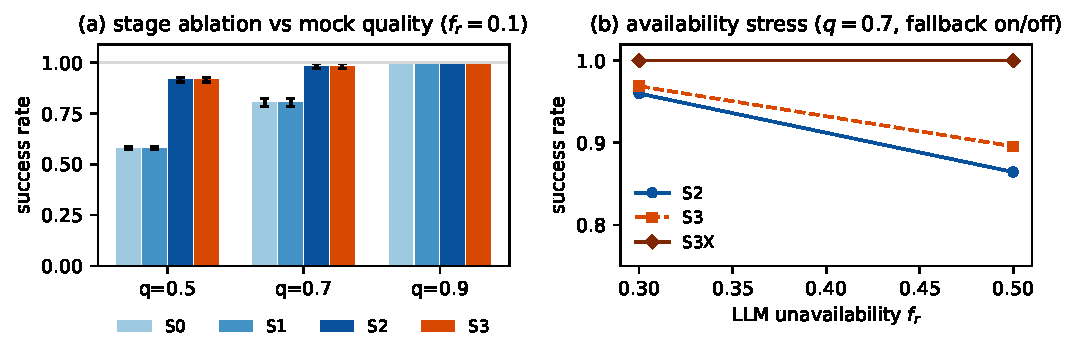
\includegraphics[width=\linewidth]{figures/fig_ablation.pdf}
\caption{Architectural ablation (mock LLM, seeded, 150 tasks $\times$ 3 seeds). (a)~Success rate by pipeline stage and injected quality. (b)~Availability stress isolating the fallback layer (narrow vs.\ full template coverage: S3 vs.\ S3X).}
\label{fig:ablation}
\end{figure}

\subsection{Instrumented Failure Taxonomy}\label{sec:taxonomy}

The v1.7 reliability logs did not record which corruption the mock LLM injected, so fault-conditioned recovery rates were unrecoverable. We re-run the benchmark with call-level instrumentation logging every generation and healing call ($353$ injected faults across $q \in \{0.5,0.7,0.9\}$, 3 seeds, 200 tasks/run). Recovery is remarkably uniform across corruption classes (Fig.~\ref{fig:taxonomy}): syntax errors $82.5\%$ [$76.1, 87.4$] (Wilson 95\%), name errors $87.7\%$, runtime division faults $86.4\%$, and import-whitelist violations $86.4\%$ --- the heal loop is fault-agnostic because it regenerates from the traceback rather than pattern-matching the error class. With $n{=}200$ per level the end-to-end success rate at $q=0.5$ is $91.7\%$ [$89.2, 93.6$], refining the v1.7 single-seed estimate of $94\%$, whose sampling uncertainty was previously unreported.

\begin{figure}[H]
\centering
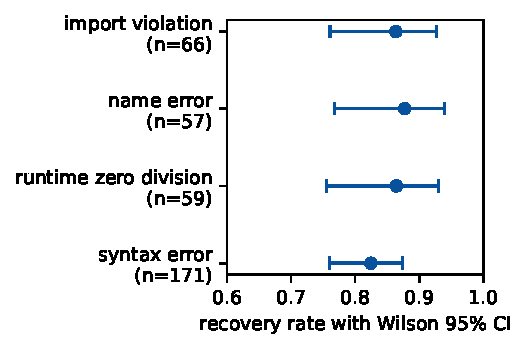
\includegraphics[width=0.6\linewidth]{figures/fig_failure_taxonomy.pdf}
\caption{Injected-fault recovery rates with Wilson 95\% CIs (353 faults).}
\label{fig:taxonomy}
\end{figure}

\subsection{Towards an End-to-End Reliability Calculus}\label{sec:calculus}

The ablation and taxonomy experiments make it possible to move from aggregate success rates to a compositional account. Because the pipeline's outcome paths are mutually exclusive by construction, end-to-end reliability decomposes \emph{exactly} as the chain rule over its sequential gates,
\begin{equation}
R_{\mathrm{end}}
= P(\mathrm{first\_pass})
+ P(\mathrm{enter\ heal})\cdot\rho_{\mathrm{heal}}
+ P(\mathrm{enter\ fallback})\cdot\rho_{\mathrm{fb}},
\label{eq:composition}
\end{equation}
with no independence assumption needed for the identity itself. Independence enters only when one tries to \emph{predict} the stage conditionals from marginals --- and there it fails measurably. Under a naive model granting the healing loop four independent generation attempts at per-call quality $q$, one expects $\rho^{\mathrm{ind}}_{\mathrm{heal}} = 1-(1-q)^{4}$, i.e.\ $93.8\%$ at $q=0.5$; the measured value is $81.5\%$ (Table~\ref{tab:calculus}). We call this gap a \emph{correlation penalty}: the healer draws from the same degraded LLM that produced the fault, so residual failures concentrate exactly on tasks whose healing calls are also corrupted. Reliability therefore does not compose multiplicatively across stages that share a component --- it must be designed in, e.g.\ through fallback diversity or heterogeneous heal models.

\begin{table}[H]
\centering
\caption{Reliability composition: exact path decomposition vs.\ naive independence prediction (S2 pipeline, 450 tasks per row). $\rho_{\mathrm{heal}}$ is recovery conditional on entering healing.}
\label{tab:calculus}
\small
\begin{tabular}{@{}lcccccc@{}}
\toprule
$q$ & first\_pass & enter heal & healed & failed & $\rho_{\mathrm{heal}}$ measured & $1-(1-q)^{4}$ \\
\midrule
0.5 & 54.4\% & 45.6\% & 37.1\% & 8.4\% & 81.5\% & 93.8\% \\
0.7 & 79.3\% & 20.7\% & 18.9\% & 1.8\% & 91.4\% & 99.2\% \\
\bottomrule
\end{tabular}
\end{table}

The encoding/hardware factor behaves differently. Channel distortion arises from device physics and is statistically independent of software-side orchestration failures, so composing pipeline reliability with a placement-dependent fidelity factor ($F_{\mathrm{hw}} = 1.00$ point-wise on calibrated layouts vs.\ $0$ at extreme weights under adversarial placement; Section~\ref{sec:sweep}) is empirically justified --- but only \emph{conditional on a pinned, calibration-checked layout}. Enforcing exactly that condition is the middleware's job; without calibration-aware layout as a first-class contract, no end-to-end guarantee survives contact with a badly-placed circuit.

With full template coverage the fallback stage reaches $\rho_{\mathrm{fb}} = 100\%$ ($79/79$ recoveries across all availability-stress runs), which closes Eq.~\eqref{eq:composition} to $R_{\mathrm{end}} = 100\%$ under pure unavailability stress at $q = 0.7$: every generation failure is absorbed by the deterministic layer. The observed limits of end-to-end reliability are thus (i) correlated LLM faults surviving healing ($8.4\%$ at $q=0.5$) and (ii) hardware placement outside tolerance --- both of which the middleware can measure, and the second of which it can eliminate by construction.

\subsection{Limitations of Current Evaluation}

We are transparent about what this evaluation does \textbf{not} demonstrate:

\begin{enumerate}[leftmargin=2em]
    \item \textbf{Physical QPU validation is placement-scoped, not device-wide.} Section~\ref{sec:qpu} shows the bare encoding meets the $0.05$ tolerance on a well-calibrated pinned qubit ($0.028$) but fails by $\sim$4$\times$ on an adversarially chosen bad one ($0.213$), so end-to-end fidelity guarantees require calibration-aware layout enforcement for \emph{arbitrary} placements; zero-noise extrapolation and deeper mitigation remain unintegrated, results are from one device on one day (three repeat jobs per cell), and cross-day drift is unquantified.
    \item \textbf{No cross-framework usability comparison.} We have not compared UniMind against PennyLane/Qiskit in terms of usability or feature completeness.
    \item \textbf{No real-API LLM measurements.} The reliability benchmark uses an injectable mock LLM; pass@$k$ rates and token consumption on a real model remain to be measured (Section~\ref{sec:llm_rel}).
    \item \textbf{Scalability on physical devices.} The 1:1 bit-to-qubit mapping and single-shot-based orchestration have not been exercised beyond a 10-qubit simulated circuit.
\end{enumerate}


\section{Discussion}\label{sec:discussion}

\subsection{Implications for Quantum-Ready AI Middleware}

The UniMind architecture illustrates three design principles:

\begin{enumerate}[leftmargin=2em]
    \item \textbf{Classical preprocessing as a bridge.} Classical signal processing techniques can produce meaningful parameters for quantum state preparation, reducing manual circuit design.
    \item \textbf{User-space orchestration, not kernel replacement.} LLMs are powerful task planners but unsuitable as OS kernels.
    \item \textbf{Backend abstraction.} A unified API enables gradual migration as hardware matures.
\end{enumerate}

\subsection{Threats to Validity}\label{sec:threats}

\paragraph{T1: LLM hallucination.} The orchestration layer may generate semantically incorrect code. The reliability benchmark (Section~\ref{sec:llm_rel}) and its instrumented multi-seed re-run (Section~\ref{sec:taxonomy}) quantify this risk: with a mock LLM degraded to 50\% per-call quality, the self-healing loop keeps the end-to-end success rate at $91.7\%$ [$89.2, 93.6$], with residual failures concentrated where the heal step itself receives broken output (a measured correlation penalty; Section~\ref{sec:calculus}). Mitigations: constrained decoding, rule-based fallback with full template coverage (measured at $100\%$ recovery under availability stress), and human-in-the-loop review.

\paragraph{T2: Quantum noise sensitivity.} The encoding assumes ideal gates. Section~\ref{sec:noise} quantifies the degradation: the $\theta_i = 2\arcsin(\sqrt{w_i})$ mapping is symmetric-sensitive under depolarizing noise (deviation $\approx p\,|1-2w|$; $w=0.5$ essentially immune) and one-sided-sensitive under $T_1$ damping (high weights decay toward $|0\rangle$), with the $0.05$ tolerance broken at $\gamma \approx 5\mathrm{e}{-2}$. Future work will integrate zero-noise extrapolation.

\paragraph{T3: Encoding overhead.} The 1:1 bit-to-qubit mapping is qubit-inefficient. Future benchmarks will quantify the latency trade-off between LLM-orchestrated generation and direct API calls, measuring tokens consumed and circuit depth overhead.

\paragraph{T4: Security of LLM-generated code.} Executing dynamic code carries injection risks. The sandbox security evaluation (Section~\ref{sec:security}) shows 20 of 21 escape attempts blocked by a three-layer restricted namespace; the one unblocked case (object-graph traversal) cannot be weaponized into process or file access. Full OS-level sandboxing (process-level isolation) is intentionally not implemented and remains outside the prototype's scope.

\paragraph{T5: Evaluation scope.} Physical-QPU validation is now performed with placement control (Section~\ref{sec:qpu}): the bare encoding meets tolerance on a calibrated pinned qubit and fails on an adversarially chosen one, so fidelity conclusions are conditional on layout; the most significant remaining evaluation gap is calibration-aware layout enforcement across arbitrary placements, integration of deeper error mitigation (zero-noise extrapolation, T-REx), cross-framework comparison, and cross-day drift quantification.

\paragraph{T6: New threats introduced by the v2.0 experiments.} All QPU results in Section~\ref{sec:qpu} are from one device (\texttt{ibm\_marrakesh}) captured on one day (2026-08-23) with three repeat jobs per cell; cross-day drift is unquantified. Qubit~37 is an adversarially selected extreme ($82\%$ total readout error); typical device medians are far better ($2.3\%$). The v1.7 jobs' physical placements cannot be recovered retroactively, so the ``placement artifact'' explanation of the v1.7 distortion, while consistent with every measurement here, is not uniquely provable. Mock-LLM quality $q$ is a synthetic parameter defining a generation policy, not real-API behaviour; the ablation and taxonomy results therefore quantify architecture-level contributions under controlled degradation, not absolute production reliability.

\subsection{Roadmap for Quantum-Ready AI Middleware}\label{sec:roadmap}

\paragraph{Phase 1: Functional validation (2024--2026).} Completed in this revision: end-to-end baseline comparison against bare Qiskit and a rule-based dispatcher (Section~\ref{sec:baseline}), LLM reliability evaluation (Section~\ref{sec:llm_rel}), fault-injection analysis (Section~\ref{sec:fault}), noise-sensitivity quantification (Section~\ref{sec:noise}), sandboxed execution with a security evaluation (Section~\ref{sec:security}), and physical QPU validation on \texttt{ibm\_marrakesh} (Section~\ref{sec:qpu}). Outstanding: cross-framework comparison with PennyLane/Qiskit and hardware-level error mitigation.

\paragraph{Phase 2: NISQ integration (2026--2030).} Integrate error mitigation. Implement sandboxed execution. Standardize middleware APIs.

\paragraph{Phase 3: Fault-tolerant era (2030+).} Adapt to error-corrected hardware. Explore qubit-efficient encoding. Support distributed quantum clusters.


\section{Conclusion and Future Work}\label{sec:conclusion}

This paper presented UniMind, a middleware framework for bridging classical AI workloads and quantum computing backends. We validated the framework with reproducible experiments: mathematical correctness (maximum $\langle Z \rangle$ deviation of $0.0110$ across 8192 shots), system performance (up to $10.9\times$ acceleration via vectorized C-backend execution and $4.5\times$ end-to-end speedup via Rust FFI, with a component-level breakdown attributing residual overhead to Python-side normalization and marshaling), a three-arm baseline comparison in which only the UniMind pipeline covered all five task classes while enforcing code safety, an LLM-reliability benchmark showing 91.7--100\% success across injected quality levels with Wilson-quantified uncertainty and 100\% rejection of adversarial intents, fault-injection analysis recovering four of five failure classes with uniformly measured per-fault recovery rates (82--88\%), a component ablation attributing the reliability gains to self-healing ($+34$ points at $q{=}0.5$) with fallback reaching $100\%$ recovery under availability stress once template coverage is complete, a noise-sensitivity study quantifying the encoding's operating envelope, a sandbox security evaluation blocking 20 of 21 escape attempts, and placement-controlled physical QPU sweeps on \texttt{ibm\_marrakesh}: the bare encoding meets the $0.05$ tolerance on calibrated layouts (max deviation $0.028$) while adversarial placement inflates distortion to $0.213$, revising our earlier conclusion --- encoding fidelity on real hardware is placement-dominated, not mitigation-limited.

We acknowledge the remaining limitations: deeper error mitigation (zero-noise extrapolation, T-REx) on hardware, cross-framework usability comparison, and real-API token accounting. The fault-injection study additionally exposed a concrete robustness defect---an unguarded hardware-monitor call in the orchestrator's success path---which is the immediate target of the next revision. Future work will prioritize zero-noise extrapolation on hardware, process-level sandbox isolation, and validation on error-corrected hardware.

More broadly, quantum-ready computing requires not only hardware advances but also new software abstractions; UniMind represents an early step toward a middleware layer that reduces the friction between classical AI intent and quantum hardware execution.


\newpage
\begin{thebibliography}{14}

\bibitem{biamonte2017}
J.~Biamonte, P.~Wittek, N.~Pancotti, P.~Rebentrost, N.~Wiebe, and S.~Lloyd,
``Quantum machine learning,''
\textit{Nature}, vol.~549, no.~7671, pp.~195--202, 2017.

\bibitem{preskill2018}
J.~Preskill,
``Quantum Computing in the NISQ era and beyond,''
\textit{Quantum}, vol.~2, p.~79, 2018.

\bibitem{cerezo2021}
M.~Cerezo et al.,
``Variational quantum algorithms,''
\textit{Nature Reviews Physics}, vol.~3, no.~9, pp.~625--644, 2021.

\bibitem{havlicek2019}
V.~Havl\'{i}\v{c}ek et al.,
``Supervised learning with quantum-enhanced feature spaces,''
\textit{Nature}, vol.~567, no.~7747, pp.~209--212, 2019.

\bibitem{schuld2021}
M.~Schuld and F.~Petruccione,
\textit{Machine Learning with Quantum Computers}, 2nd~ed.
Cham, Switzerland: Springer, 2021.

\bibitem{wang2024}
L.~Wang et al.,
``A survey on large language model-based autonomous agents,''
\textit{Frontiers of Computer Science}, vol.~18, no.~6, art.~no.~186345, 2024.

\bibitem{tan2026}
Y.~X.~Tan,
``UniMind: A middleware framework for hybrid quantum-classical computing,''
GitHub Repository, 2026.
[Online]. Available: \url{https://github.com/yxtan5022-maker/unimind-os}.
[Accessed: 2026].

\bibitem{kandala2017}
A.~Kandala et al.,
``Hardware-efficient variational quantum eigensolver for small molecules and quantum magnets,''
\textit{Nature}, vol.~549, no.~7671, pp.~242--246, 2017.

\bibitem{shor1994}
P.~W.~Shor,
``Algorithms for quantum computation: discrete logarithms and factoring,''
in \textit{Proc. 35th Annual Symposium on Foundations of Computer Science},
1994, pp.~124--134.

\bibitem{tanenbaum2023}
A.~S.~Tanenbaum and H.~Bos,
\textit{Modern Operating Systems}, 5th~ed.
Hoboken, NJ, USA: Pearson, 2023.

\bibitem{microsoft2024}
Microsoft Corporation,
``Azure Quantum: Q\# and the Quantum Development Kit documentation,''
Redmond, WA, USA, 2024.
\url{https://learn.microsoft.com/azure/quantum}

\bibitem{aws2024}
Amazon Web Services,
``Amazon Braket Developer Guide,''
Seattle, WA, USA, 2024.
\url{https://docs.aws.amazon.com/braket}

\bibitem{bergholm2018}
V.~Bergholm et al.,
``PennyLane: Automatic differentiation of hybrid quantum-classical computations,''
arXiv preprint arXiv:1811.04968, 2018.

\bibitem{lu2025unimind}
W.~Lu et al.,
``UniMind: Unleashing the power of LLMs for unified multi-task brain decoding,''
arXiv preprint arXiv:2506.18962, 2025.

\end{thebibliography}


\newpage
\appendix

\section{Repository Structure}

\begingroup
\footnotesize
\begin{verbatim}
unimind-os/
|-- umos_py/           # Core Unibit engine (Python, auto-loads Rust FFI)
|-- bridge/            # AI-as-Orchestrator, rule-based fallback, self-healing
|-- quantum/           # QUnibit multi-backend quantum circuit mapping
|-- core/              # Rust-accelerated Unibit engine (FFI)
|-- kernel/            # C++ Topology Mapper (hardware detection)
|-- gui/               # Tkinter GUI
|-- experiments/       # Reproducible experiments (math verification, benchmarks,
|                      #   baseline, LLM reliability, fault injection, noise,
|                      #   security, physical QPU validation)
|-- tests/             # 47 pytest tests
|-- docs/              # Paper design spec + whitepaper
|-- example/           # Proof-of-concept demos
|-- assets/            # Supplementary assets
|-- .github/workflows/ # CI/CD pipeline (GitHub Actions)
|-- CMakeLists.txt     # C++ build configuration
|-- Makefile           # Build automation
|-- pyproject.toml     # Python package config
|-- requirements.txt   # Python dependencies (versions pinned)
|-- Dockerfile         # Multi-stage build (Rust core + Python runtime)
|-- run.py             # Main entry point
|-- build.py           # One-shot build script
\end{verbatim}
\endgroup

\section{Quick Start Commands}

\begingroup
\footnotesize
\begin{verbatim}
# Clone and install the software
git clone https://github.com/yxtan5022-maker/unimind-os.git
cd unimind-os
pip install -e .

# Run core demo and quantum circuit mapping
python run.py
pip install -e ".[quantum]"
python -c "from quantum.qunibit import demo; demo()"

# Clone the dev repo that contains the reproducible experiments
git clone https://github.com/yxtan5022-maker/unimind-dev.git
cd unimind-dev

# Reproduce the paper's experiments (seed 42, mock LLM)
python experiments/test_math_verification.py      # Table 3
python experiments/benchmark_unibit.py            # Table 4
python experiments/benchmark_breakdown.py         # Table 5
python experiments/baseline_comparison.py --llm mock # Table 6
python experiments/llm_reliability.py --mode mock # Table 7
python experiments/fault_injection.py             # Table 8
python experiments/noise_sensitivity.py           # Table 9
python experiments/security_sandbox.py            # Table 10
python experiments/qpu_validation.py --mode ideal # Table 11
python experiments/qpu_validation.py --mode fake  # Table 11
python experiments/qpu_validation.py --mode real  # Table 11 (needs token)

# Run all tests
python -m pytest tests/ -v

# Reproducible environment (Docker; requires docker installed)
docker build -t unimind-dev .
docker run --rm unimind-dev python -m pytest tests/ -q

# Build C++ kernel
cmake -S . -B build
cmake --build build --config Release

# Build Rust core
cd core && cargo build --release && cd ..

# One-shot build
python build.py
\end{verbatim}
\endgroup

\vfill
\begin{center}
\small\copyright\ 2026 Y. X. Tan. This work is licensed under CC BY 4.0; the accompanying software (\texttt{unimind-os}) is MIT-licensed.
\end{center}

\end{document}
